\section{Probabilità}

\begin{quotation}
	"Si occupa di prevedere quanto è facile/possibile che qualcosa accada. Consiste in passaggi logici rigorosi partendo da un modello fisso (spazio di probabilità)."
\end{quotation}

\definizione{Fenomeno}{Un fenomeno è qualcosa che acacde e che porta ad'un esito o risultato.}{d:fenomeno}

Un fenomeno può essere:
\begin{itemize}
	\item \textbf{Deterministico} se il risultato può essere predetto con esattezza.
	\item \textbf{Aleatorio} se il risultato è imprevedibile.
\end{itemize}

\definizione{Evento}{Un evento è un insieme di possibili risultati.}{d:evento}

\definizione{Valutazione di probabilità}{La valutazione di probabilità è una funzione che ad'ogni evento associa un numero tanto più grande quanto riteniamo che l'evento possa accadere.}{d:valProb}

\definizione{Evento coerente}{Sia $\Omega$ l'insieme dei risultati. Un evento è un sotto insieme di $\Omega$ di cui ha senso calcolare la valutazione di probabilità, ossia:
\begin{enumerate}
	\item Se $A_1,\dots$ sono eventi allora $\bigcup_i A_i$ è un evento.
	\item Se $A$ è un evento allora $A^C$ è un evento.
	\item $\Omega$ è un evento ($\Omega \in \mathscr{A}$).
\end{enumerate}}{d:eventoProb}

\osservazione{Una collezione di sotto insiemi di $\omega$ che soddisfa tutti i presupposti si dice \textbf{famiglia coerente d'eventi}, con simbolo $\mathscr{A}$.}

\osservazione{Non tutti i sotto insiemi di $\Omega$ sono eventi.}

La valutazione di probabilità, $P$, $P:\mathscr{A}\to\mathbb{R}_{\geqslant0}$, deve soddisfare le proprietà:
\begin{enumerate}
	\item $P(\Omega)=1$.
	\item $P(A)\geqslant0,\forall \ evento \ A$.
	\item Se $A_1,\dots$ sono eventi disgiunti allora \[P(\bigcup_{i=1}^\infty A_i)=\sum_{i=1}^\infty P(A_i)\]
\end{enumerate}

\osservazione{$P$ non ha dominio $\Omega$ ma l'insieme degli eventi. Non calcoliamo la $P$ di un risultato ma di un evento.}

\definizione{Probabilità uniforme}{
La probabilità è uniforme se:
\begin{enumerate}
	\item Se $\Omega$ è finito con $|\Omega|=n$.
	\item Se ogni sotto insieme di $\Omega$ è un evento.
	\item Se $\omega_1$ e $\omega_2$ sono due risultati allora $P(\{\omega_1\})=P(\{\omega_2\})$.
\end{enumerate}

Dalle proprietà della valutazione di probabilità deduciamo anche \[P(\omega_1)+\dots+P(\omega_n)=P(\Omega)=1\]

In generale abbiamo quindi \[P(\omega)=\frac{1}{n}, \forall \omega \in \Omega\]
}{d:probUnif}

\definizione{Probabilità eventi}{Sia $A \in \Omega, A=\{\omega_1,\dots,\omega_k\}$ \[P(A)=\frac{|A|}{|\Omega|}=\frac{\#risultati favorevoli}{\#risultati possibili}\]}{d:probEv}

Ragionamento: $P(A)=P(\omega_1)+\dots+P(\omega_k)=\frac{1}{n}+\dots+\frac{1}{n}=\frac{k}{n}$, se $|A|=k$.

\osservazione{Vale uno spazio con proprietà uniforme.}

\definizione{Non-esempio}{Un non-esempio è qualcosa che non funziona.}{d:nonEsempio}

\mysubsection{Considerazioni elementari}
\begin{itemize}
	\item Se $E$ è un evento allora $E^C$ è un evento.
	\item $E\cup E^C=\Omega$ è un uninoe disguinta.
	\item Se $P(E)+P(E^C)=1$ allora $P(E^C)=1-P(E)$.
\end{itemize}

\osservazione{Il principio di inclusione-esclusione vale anche per l'unione di più di due probabilità.}

\definizione{Probabilità condizionata}{Chiamiamo probabilità condizionata la probabilità che accada l'evento $B$ sapendo che accade l'evento $A$ prima di $B$.\[P(B\mid A)=\frac{P(A\cap B)}{P(A)}\]}{d:probCond}

In altre parole riparametrizziamo la probabilità di $B$ da $\Omega$ al sotto insieme codiviso con $A$.

\osservazione{Ponendo $P'(B)=P(B\mid A)$ allora $P'$ soddisfa le proprietà delle valutazioni di probabilità:
\begin{itemize}
	\item $P'(\Omega)=P(\Omega\mid A)=\frac{P(\Omega \cap A)}{P(A)}=1$.
	\item $P'(A_1\cup A_2)=P'(A_1)+P'(A_2)$ se $A_1,A_2$ sono disgiunti.
\end{itemize}}
\osservazione{$P(A\cap B)=P(B\mid A)P(A)$.}

\definizione{Formula delle probabilità totali}{Sia $\Omega$ partizionato in $\{A_1,A_2,\dots\}$. Per sapere la probabilità d'un evento $B$ condizionato da un qualsiasi altro evento. \[P(B)=\sum_{i=1}^nP(B\cap A_i)=\sum_{i=1}^nP(B\mid A)P(A)\]}{formulaPorblTot}

\definizione{Formula di Bayes}{Siano $A,B$ eventi. \[P(B\mid A)=\frac{P(A\mid B)P(B)}{P(A)}\]}{d:fBaeys}

\dimostrazione{d:fBaeys}{Siano $P(A\mid B)=\frac{P(A\cap B)}{P(B)}$ e $P(B\mid A)=\frac{P(A\cap B)}{P(A)}$. Allora $P(A\cap B)=P(A\mid B)P(B)=P(B\mid A)P(A)=P(A  \cap B)$.}

\definizione{Eventi indipendenti}{$A$ e $B$ sono eventi indipendenti se sapere che accade uno dei due non cambia la probabilità che accada l'altro. \[P(B\mid A)=P(B)\] \[P(A\mid B)=P(A)\]}{d:evDip}

Dato che $P(A\mid B)=\frac{P(A\cap B)}{P(B)}=P(A)$ allora $P(A\cap B)=P(A)P(B)$.

\definizione{Variabili Aleatorie}{Sia $\Omega$ uno spazio di probabilità, $A$ un insieme coerente di eventi e $P$ la valutazione di probabilità.

Una \textbf{variabile aleatoria} è una funzione $X:\Omega\to\mathbb{R}$ tale che $\forall a \in \mathbb{R}, \{\omega\in\Omega\mid X(\omega)\leqslant a\}$, oppure $X\leqslant a$, deve essere un evento. (si scrive anche $\chi_A$).}{d:varAleatoria}

Per una variabile aleatoria non ha senso scrivere $P(X)$, ma ha senso scrivere $P(X\leqslant a)$.
Una variabile aleatoria può essere continua o discreta.

\definizione{Funzione di ripartizione}{Sia $X$ una variabile aleatoria. La sua funzione di ripartizione $F_X$ è una funzione $F_X:\mathbb{R}\to\mathbb{R}$ definita come $F_X(t)=P(X\leqslant t)$.}{d:fRipartizione}

\definizione{Densità concreta discreta}{Sia $X$ una variabile aleatoria discreta.
La densità concreta discreta di $X$ è $dx:\mathbb{R}\to\mathbb{R}$ con \[dx(h)=P(X=h)=
\begin{cases}
	a_1 \ se\ h=0,\dots \\
	\dots \\
	0 \ altrimenti
\end{cases}\] La densità concreta discreta soddisfa le proprietà:
\begin{enumerate}
	\item $dx(h)\geqslant0,\forall h$.
	\item $dx(h)\ne0$ per una quantità finita o numerabile di valori $h$.
	\item $\sum_hdx(h)=1$.
\end{enumerate}}{d:densConc}

\osservazione{Una densità è valida se soddisfa le tre proprietà.}

\definizione{Densità astratta discreta}{Sia $X$ una variabile aleatoria discreta. La densità astratta discreta è $d:\mathbb{R}\to\mathbb{R}$ e soddisfa le proprietà:
\begin{enumerate}
	\item $d(h)\geqslant0,\forall h$.
	\item $d(h)\ne0$ per una quantità discreta di valori $h$.
	\item $\sum_hd(h)=1$.
\end{enumerate}}{d:denAst}

\mysubsection{Approfondimento Serie Geometrica}
Sia $0<a<1$ allora $1-a^n=(1-a)(1+\dots+a^{n-1})$ sapendo che $(1+\dots+a^{n-1}=\frac{1-a^n}{1-a}$ possiamo dire che \[\lim\limits_{h\to\infty}(1+\dots+a^{n-1})=\lim\limits_{h\to\infty}\frac{1-a^n}{1-a}=\frac{1}{1-a}=\sum_{h=0}^\infty a^h\]

\definizione{Densità uniforme}{Sia $X$ una v.a., si dice uniforme nell'insieme $A=\{a_1,\dots,a_n\}\subseteq\mathbb{R}$ se \[dx(h)=
\begin{cases}
	\frac{1}{n} \ se \ h=a_1,\dots,a_n\\
	0 \ altrimenti
\end{cases}\]

Si scrive $X\sim U(\{\dots\})$.}{d:densUnif}

\definizione{Densità di Bernulli}{Si dice densità di Bernulli se $X$ assume solo i valori 0 e 1. \[dx(h)=
\begin{cases}
	p \ se \ h=1\\
	1-p \ se \ h=0\\
	0 \ altrimenti
\end{cases}\]

Si scrive $X\sim B(1,p)$.}{d:densBern}

\osservazione{Si usa quando qualcosa può accadere o non accadere.}

\definizione{Schema successo insuccesso}{Lo schema successo insuccesso è una sequenza di $n$ fenomeni aleatori ognuno dei quali da un successo oppure un insuccesso.}{d:ssi}

\definizione{S.S.I. a prove indipendenti}{Uno schema successo insuccesso si dice a prove indipendenti se:
\begin{enumerate}
	\item Ogni prova ha la stessa probabilità di dare successo.
	\item L'esito di ogni tentativo è indipendente da quello degl'altri.
\end{enumerate}

La variabile $X=\# successi$ la chiamiamo binomiale e scriviamo $X\sim B(h,p)$ con $h$ il numero di tentativi e $p$ la probabilità che ogni tentativo dia successo.

\[dx(k)=
\begin{cases}
	\binom{h}{k}p^k(1-p)^{h-k} \ se \ k=1,\dots,n\\
	0 \ altrimenti
\end{cases}\]}{d:ssiProvInd}

\definizione{S.S.I. senza rimpiazzo}{Sia $\Omega=$ le combinazioni, con probabilità uniforme, di $n$ palline tra blu e rosse, $|\Omega|=\binom{b+r}{n}$.
Uno s.s.i. si dice senza rimpiazzo se:
\begin{enumerate}
	\item L'ordine delle estrazioni non è importate.
	\item Ogni prova non ha la stessa probabilità di dare successo.
	\item L'esito di ogni tentativo non è indipendente da quello degl'altri.
\end{enumerate}

La variabile $X=\# successi$ (estrazione pallina blu) la chiamiamo ipergeometrica. Scriviamo $X\sim H(h,b,r)$ con $h$ il numero di tentativi.

I risultati favorevoli a "$X=k$" sono $\binom{b}{k}\cdot\binom{r}{h-k}$ ossia la scelta di $k$ palline blue per la scelta di $h-k$ palline rosse.

\[P(X=k)=dx(k)=
\begin{cases}
	\frac{\binom{b}{k}\cdot\binom{r}{h-k}}{\binom{b+r}{h}} \ se \ k=0,\dots,n\\
	0 \ altrimenti
\end{cases}\]}{d:ssiSenzaRimpiazzo}

\definizione{Variabili tempo di primo successo}{Sia $\Omega=$ le combinazioni, con probabilità uniforme, di $n$ palline tra blu e rosse, $|\Omega|=\binom{b+r}{n}$.
Si parla di variabile tempo di primo successo quando estraiamo senza rimpiazzo fino ad'ottenere un successo (blu).

Definiamo $T=\#$tentativi effettuati.
Il tempo di primo successo in uno s.s.i. a prove indipendenti definisce:
\begin{enumerate}
	\item $T$=Tempo primo successo che assume $\infty$ valori.
	\item $p$=Probabilità di avere successo ad'ogni tentativo.
\end{enumerate}

\[p(T=k)=(1-p)^{k-1}p\]

\[d_T(k)=
\begin{cases}
	(1-p)^{k-1}p \ se \ k=1,\dots\\
	0 \ altrimenti
\end{cases}\]

Diciamo $T\sim \tilde{G}(p)$, ossia $T$ ha densità geometrica modificata di parametro $p$.
Siccome $d_T$ è una densità abbiamo:

\[\sum_{k=1}^\infty (1-p)^{k-1}p=1\]
}{d:varTempPrimoSucc}

\definizione{Variabili geometrice non modificate}{In uno s.s.i. a prove indipendenti la variabile geometrica $X$ da il numero di fallimenti prima di un successo.

$X+1=T$ è una variabile geometrica modificata con $X$ che assume vlaori da 0 a $+\infty$. Quindi
$dx(k)=P(X=k)=P(T-1=k)=P(T=k+1)=d_T(k+1)=
\begin{cases}
	p(1-p)^k \ se \ k=0,\dots\\
	0 \ altrimenti
\end{cases}$

Scriviamo $X\sim G(p)$.}{d:varGeom}

\proprieta{Mancanza di memoria}{\[P(X\geqslant k+m\mid X\geqslant k)=P(X\geqslant m)\]}{d:mancMem}

\dimostrazione{d:mancMem}{Sia $X\sim G(p)$. Perchè $P(X\geqslant k)$ è uguale a $(1-p)^k$, ossia i primi $k$ tentativi vanno male?
\begin{align*}
	P(X\geqslant k+m\mid X\geqslant k)&=\frac{P(X\geqslant k+m \cap X \geqslant k)}{P(X\geqslant k)}\\
	&=\frac{(1-p)^{k+m}}{(1-p)^k}\\
	&=(1-p)^m\\
	&=P(X\geqslant m)
\end{align*}}

\definizione{Variabili di Poisson}{Una variabile aleatoria $X$ si dice variabile di Poisson di parametro $\lambda>0$ se ha la seguente densità: \[d(k)=
\begin{cases}
	e^{-\lambda}\frac{\lambda^k}{k!}\ k=0,\dots\\
	0 \ altrimenti
\end{cases}\]

Scriviamo $X\sim P(\lambda)$.}{d:varPoisson}

\osservazione{$d(k)$ è una densità discreta astratta:

\begin{itemize}
	\item $d(k)\geqslant0,\forall k$.
	\item $d(k)\ne0,\forall k \in \mathbb{N}$.
	\item $\sum_{k=0}^\infty d(k)=\sum_{k=0}^\infty e^{-\lambda}\frac{\lambda^k}{k!}=e^{-\lambda}\sum_{k=0}^\infty \frac{\lambda^k}{k!}=e^{-\lambda}e^\lambda=1$.
\end{itemize}}

Ricorda: $e^x=\sum_{k0=}^\infty\frac{x^k}{k!},\forall x \in \mathbb{R}$.

\teorema{Variabile di Poisson}{Sia $X$ una variabile binomiale, $X\sim B(n,p)$, e poniamo $\lambda=pn$ ottentendo $X\sim B(n, \lambda n)$.
Per $n\to\infty$ la densità di $X$ tende alla densità di Poisson $P(\lambda)$.}{t:Poisson}

\dimostrazione{t:Poisson}{La densità di $X$ è

\begin{align*}
	d_X(k) &= \binom{n}{k}\left(\frac{\lambda}{n}\right)^k\left(1-\frac{\lambda}{n}\right)^{n-k}\\
	&= \frac{n(n-1)(n-k+1)}{k!}\frac{\lambda^k}{n^k}\left(1-\frac{\lambda}{n}\right)^n\left(1-\frac{\lambda}{n}\right)^{-k}\\
	&=\underbracket{\frac{\lambda^k}{k!}}_{e^k}\underbracket{\frac{n(n-1)\dots(n-k+1)}{n^k}}_1\underbracket{\left(1-\frac{\lambda}{n}\right)^n}_{e^{-\lambda}}\underbracket{\left(1-\frac{\lambda}{n}\right)^{-k}}_1\\
	&=e^\lambda e^{-\lambda}=1
\end{align*}}

\definizione{Variabili aleatorie multidimensionali}{Una v.a. n-dimensionale è data da $(X_1,\dots,X_n)$ dove $X_1,\dots,X_n$ sono variabili aleatorie.}{d:vam}

\definizione{Variabile aleatoria bidimensionale}{Una variabile aleatoria bidimensionale $(X,Y)$ ha densità $d_{X,Y}:\mathbb{R}^2\to\mathbb{R}$.

\[d_{X,Y}(h,k)=P(X=h,Y=k)\]}{d:densitàVam2}
La densità multi dimensionale $d_{X,Y}$ si dice anche \textbf{densità congiunta}.
La densità delle variabili $X$ e $Y$ , $d_X$ e $d_Y$, si dicono \textbf{densità marginali}.

\[
\begin{array}{c|ccc}
	X \backslash Y & 0 & \dots & n\\
	\hline
	0 & n_{00} & \dots & n_{0n}\\
	\vdots & \vdots & \ddots & \vdots\\
	n & n_{n0} & \dots & n_{nn}\\
\end{array}
\quad
\begin{aligned}
	\\
	&= P(X=0)\\
	&= P(X=\dots)\\
	&= P(X=n)
\end{aligned}
\]


Le d.marginali sono univocamente determinabili dalla d.congiunta:
\[d_X(h)=\sum_kd_{X,Y}(h,k)\]
\[d_Y(k)=\sum_hd_{X,Y}(h,k)\]

Le densità marginali non determinano la densità congiunta.

\definizione{Variabili aleatorie indipendenti}{Due variabili aleatorie $X,Y$ si dicono indipendenti se

\[P(X=h,Y=k)=P(X=h)P(Y=k)\]

Ossia $d_{X,Y}(h,k)=d_X(h)d_Y(k), \forall h,k\in\mathbb{R}$.}{d:vaIndipendenti}

In altre parole $X$ e $Y$ sono indipendenti se gli eventi $"X=h"$ e $"Y=k"$ sono indipendenti per ogni $h,k$.

\definizione{Trasformazioni di variabili}{Una trasformazione di una o più variabili aleatorie è data \[\Phi(X_1,X_2), \Phi:\mathbb{R}^2\to\mathbb{R}\] oppure \[\Phi(X), \Phi:\mathbb{R}\to\mathbb{R}\]}{d:trasfVart}

\proprieta{F.r. di v.a. indipendenti}{Sia $X$ e $Y$ variabili indipendenti e $Z$ una trasformazione di variabile allora \[F_Z=F_X\cdot F_Y\]}{prop:frVAindip}
Ricorda: La funzione di ripartizione della viariabile alealtoria $X$ è $F_X(h)=P(X\leqslant h)$.

\dimostrazione{prop:frVAindip}{Sia $Z=max(X,Y)$\begin{align*}
	F_Z(k)&=P(Z\leqslant k)=P(max(X,Y)\leqslant k)\\
	&=P(X\leqslant k, Y\leqslant k)\\
	(indipendenza)&=P(X\leqslant k)P(Y\leqslant k)\\
	&=F_X(k)F_Y(k)
\end{align*}}

\proprieta{Complementare f.r. di v.a. indipendenti}{Sia $X$ e $Y$ variabili indipendenti e $Z$ una trasformazione di variabile allora \[(1-F_Z(k))=(1-F_X(k))(1-F_Y(k))\]}{prop:comfrVAindp}

\dimostrazione{prop:comfrVAindp}{Sia $Z=min(X,Y)$\begin{align*}
	1-F_Z(k)&=1-P(Z\leqslant k)\\
	&=P(Z>k)=P(min(X,Y)>k)\\
	&=P(X>k, Y>k)\\
	(indipendenza)&=P(X>k)P(Y>k)\\
	&=(1-F_X(k))(1-F_Y(k))
\end{align*}}

\definizione{Densità di una Trasformazione}{Sia $X$ una variabile aleatoria e $\Phi(X), \Phi:\mathbb{R}\to\mathbb{R}$ allora la densità della trasformazione è \[d_{\Phi(X)}(k)=\sum_{h\mid \Phi(h)=k}d_X(h)\]
per una variabile bidimensionale \[d_{\Phi(X,Y)}(k)=\sum_{i,j\mid\Phi(i,j)=k}d_{X,Y}(i,j)\]}{d:densTras}

\definizione{Valore atteso}{Il valore atteso di $X$ è \[E[X]=\sum_hd_X(h)h\]

Detto anche media o speranza matematica.}{d:valAtesso}

\proprieta{Valore atteso}{Sia $X$ variabile aleatoria e $\Phi:\mathbb{R}\to\mathbb{R}$ allora \[E[\Phi(X)]=\sum_h\Phi(h)d_X(h)\]

Analogamente \[E[\Phi(X,Y)]=\sum_{h,k}\Phi(h,k)d_{X,Y}(h,k)\]}{prop:valAtteso}

\teorema{Linearità Valore Atteso}{Il valore atteso è lineare \[E[aX+bY]=aE[X]+bE[Y]\]}{teo:linVarAtt}

\dimostrazione{teo:linVarAtt}{Sia $\Phi(X,Y)=aX+bY$ per la formula analoga della proprità del valore atteso.

\begin{align*}
	E[aX+bY]&=\sum_{h,k}(ah+bk)d_{X,Y}(h,k)\\
	&=\sum_{h,k}ahd_{X,Y}(h,k)+\sum_{h,k}bkd_{X,Y}(h,k)\\
	&=a\sum_hh\underbracket{\sum_kd_{X,Y}(h,k)}_{d_{X}(h)}+b\sum_kk\underbracket{\sum_hd_{X,Y}(h,k)}_{d_Y(k)}\\
	&=a\sum_hhd_X(h)+b\sum_kkd_Y(k)\\
	&=aE[X]+bE[Y]
\end{align*}}

\corollario{1 - Linearità valore atteso}{Sia $X\sim B(n,p)$\[E[X]=np\]}{cor:linValAtt1}

\dimostrazione{cor:linValAtt1}{Sia $X=X_1+\dots+X_n$ con $X_i\sim B(1,p), \forall i \in \{1,\dots,n\}$. Per esempio \[X_1=\begin{cases}
		1 \ \text{se esistono tenteativi che danno successo}\\
		0 \ \text{se da insuccesso}
\end{cases}\]
Per linearità $E[X]=E[X_1]+\dots+E[X_n]=p+\dots+p=np$.}

\corollario{2 - Linearità valore atteso}{Sia $X\sim H(n,b,r)$\[E[X]=n\frac{b}{b+r}\]}{cor:linValAtt2}

\dimostrazione{cor:linValAtt2}{Sia $X=X_1+\dots+X_n$ con $X_i\sim B(1,p), \forall i \in \{1,\dots,n\}$. Per esempio \[X_1=\begin{cases}
	1 \ \text{se i-esima è blu}\\
	0 \ \text{se i-esima è rossa}
\end{cases}\]
Per linearità $E[X]=E[X_1]+\dots+E[X_n]=\frac{b}{b+r}+\dots+\frac{b}{b+r}=n\frac{b}{b+r}$.}

\corollario{3 - Linearità valore atteso}{Sia $X\sim P(\lambda)$\[E[X]=\lambda\]}{cor:linValAtt3}

\definizione{Valore atteso di Variabile geometrica}{Sia $X\sim \tilde{G}(p)$.\[E[X]=\frac{1}{p}\]}{d:valAttVarGeom}

\dimostrazione{d:valAttVarGeom}{Sapendo che $d_X(k)=p(1-p)^{k-1}$ e usando il "trucchetto" ($0<x<1$)

\[\sum_{k=0}^\infty x^k=\frac{1}{1-x}\stackrel{derivo}{\to}\sum_{k=1}^\infty kx^{k-1}=\frac{1}{(1-x)^2}\]

Ponendo $x=1-p$ ottengo

\begin{align*}
	E[X]&=\sum_{k=1}^\infty kp(1-p)^{k-1}\\
	&=p\sum_{k=1}^\infty k(1-p)^{k-1}=p\frac{1}{(1-(1+p))^2}\\
	&=\frac{1}{p}
\end{align*}}

\definizione{V.a. di Variabile geometrica modificabile}{Sia $X\sim G(p)$ ossia $X+1\sim \tilde{G}(p)$\[E[X+1]=E[X]+1=\frac{1-p}{p}\]}{d:valAttGeomMod}

\definizione{Prodotto valore atteso di v.a. indipendenti}{Siano $X$ e $Y$ sono indipendenti allora \[E[XY]=E[X]E[Y]\]}{d:prodValAsoluto}
Nota: Se $X\sim B(1,p)$ ho $E[XY]=E[X^2]=E[X]=p$. Perchè $X$ vale solo 0 o 1.

\dimostrazione{d:prodValAsoluto}{Sia $\Phi(X,Y)=XY$.
\begin{align*}
	E[XY]&=\sum_{h,k}\Phi(h,k)d_{X,Y}(h,k)\\
	&=\sum_{h,k}hkd_X(h)d_Y(k)\\
	&=\sum_hhd_X(h)\sum_kkd_Y(k)\\
	&=E[X]E[Y]
\end{align*}}

Attenzione non vale il viceversa.
La definizione può valere anche se le v.a. non sono indipendenti ma \textbf{incorrelate}.

\definizione{ del valore atteso}{La varianza del valore atteso è il valore atteso dei quadrati degli scarti rispetto al valore atteso di $X$. \[\mathrm{Var}(X)=E[(X-E[X])^2]\]}{d:varValAtt}

\proprieta{Semplificazione Varianza v.a.}{\[\mathrm{Var}(X)=E[X^2]-E[X]^2\]}{prop:semplvva}

\dimostrazione{prop:semplvva}{
\begin{align*}
	\mathrm{Var}(X)&=E[(X-E[X])^2]\\
	&=E[X^2-2E[X]X+E[X]^2]\\
	&=E[X^2]-2E[X]E[X]+E[X]^2\\
	&=E[X^2]-E[X]^2
\end{align*}}

\proprieta{Varianza 1}{\[\mathrm{Var}(aX)=a^2\mathrm{Var}(X)\]}{prop:var1}

\dimostrazione{prop:var1}{
\begin{align*}
	\mathrm{Var}(aX)&=E[(aX)^2]-E[aX]^2\\
	&=a^2E[X^2]-a^2E[X]^2\\
	&=a^2(E[X^2]-E[X]^2)\\
	&=a^2\mathrm{Var}(X)
\end{align*}}

\proprieta{Varianza 2}{Siano $X$ e $Y$ variabili aleatorie indipendenti. \[\mathrm{Var}(X+Y)=\mathrm{Var}(X)+\mathrm{Var}(Y)\]}{prop:var2}

\dimostrazione{prop:var2}{
\begin{align*}
	\mathrm{Var}(X+Y)&=E[(X+Y)^2]-E[X+Y]^2\\
	&=E[X^2+2XY+Y^2]-(E[X]+E[Y])^2\\
	&=\underline{E[X^2]}+\underbracket{\cancel{2E[XY]}}_{2E[X]E[Y]}+\uuline{E[Y^2]}-\underline{E[X]^2}-\cancel{2E[X]E[Y]}-\uuline{E[Y]^2}\\
	&=\underline{\mathrm{Var}(X)}+\uuline{\mathrm{Var}(Y)}
\end{align*}}

\corollario{Varianza v.a. Binomiale}{Sia $X\sim B(n, p)$. \[\mathrm{Var}(X)=np(1-p)\]}{cor:varianza}

\dimostrazione{cor:varianza}{Sia $X=X_1+\dots+X_n$ con $X_i\sim B(1,p), \forall i \in 1,\dots,N$ indipendenti. Sia la varianza di una variabile aleatoria di bernulli $p(1-p)$.
\begin{align*}
	\mathrm{Var}(X)&=\mathrm{Var}(X_1)+\dots+\mathrm{Var}(X_n)\\
	&=p(1-p)+\dots+p(1-p)\\
	&=np(1-p)
\end{align*}}

Attenzione: Questo ragionamento non vale per $X\sim H(n,b,r)$. Infatti in questo caso possiamo scrivere $X=X_1+\dots+X_n$ con $X\sim B(1, \frac{b}{b+r})$.
Ma le $X_i$ sono indipendenti.

Se $X\sim P(\lambda)$ ossia $X\sim B(n, \frac{\lambda}{n})$ per $n\to\infty$ si ha $\mathrm{Var}(X)=\lambda$.

\teorema{Disuguaglianza di Chebyshev}{Sia $X$ una variabile aleatoria discreta, allora $\forall \epsilon>0$ \[P(|X-E[X]|>\epsilon)\leqslant\frac{\mathrm{Var}(X)}{\epsilon^2}\]}{teo:Chebyshev}

\dimostrazione{teo:Chebyshev}{Sia $A="|X-E[X]|>\epsilon"$ la distanza di $X$ dal valore atteso di $\epsilon$. \[\chi_A=\begin{cases}
	1 \ se \ A \ accade\\
	0 \ se \ A \ non \ accade
\end{cases}\]
Siano $Y=\epsilon^2\chi_A$ e $Z=(X-E[X])^2$.
Se $Y=\epsilon^2$ vuol dire che $\chi_A=1$ e quindi $|X-E[X]|>\epsilon$. Quindi $Y<Z$.
Se $Y=0$ e quindi $Y\leqslant Z$. In tutti i casi $Y\leqslant Z$ si ha $E[Y]\leqslant E[Z]$.
\[E[Y]=\epsilon^2P(|X-E[X]|>\epsilon)\]
\[E[Z]=\mathrm{Var}(X)\]
}

\definizione{Convergenza}{Sia $X_1,\dots$ una successione di variabili aleatorie. Diciamo che questa successione converge in probabilità ad $l$ se $\forall \epsilon>0$\[\lim\limits_{n\to\infty}P(|X_n-l|>\epsilon)=0\]}{d:convergenza}

\teorema{Legge dei grandi numeri}{Sia $X_1,\dots$ una successione di variabili aleatorie discrete aventi tutte la stessa densità e indipendenti.
Sia $\mu=E[X_1]$.

Poniamo $\overline{X_n}=\frac{X_1+\dots+X_n}{n}$. Allora la successione $\overline{X_n}$ converge in probabilità a $\mu$.}{teo:Gnum}

Esempio: Lancio un dato $n$ volte e $k$ è il numero di volte in cui abbiamo ottenuto 6.
Consideriamo $\frac{k}{n}$. Per $n$ piccolo questo rapporto può variare ma se $n$ è grande ci aspettiamo che sia vicino a $\frac{1}{6}$.

\dimostrazione{teo:Gnum}{Applichiamo la disuguaglianza di Chebyshev alla variabile $\overline{X_n}$.
\[P(|\overline{X_n}-E[\overline{X_n}]|>\epsilon)<\frac{\mathrm{Var}(\overline{X_n})}{\epsilon^2}\]
Siano:
\begin{enumerate}
	\item \begin{align*}
		E[\overline{X_n}]&=E\left[\frac{X_1+\dots+X_n}{n}\right]\\
		&=\frac{1}{n}(E[X_1])+\dots+E[X_n]=\mu
	\end{align*}
	\item \begin{align*}
		\mathrm{Var}(\overline{X_n})&=\mathrm{Var}\left(\frac{X_1+\dots+X_n}{n}\right)\\
		&=\frac{1}{n^2}(\mathrm{Var}(X_1)+\dots+\mathrm{Var}(X_n))\\
		&=\frac{1}{n^2}n\mathrm{Var}(X_1)=\frac{\mathrm{Var}(X_1)}{n}
	\end{align*}
\end{enumerate}


Sostituendo otteniamo

\[P(|\overline{X_n}-\mu|>\epsilon)<\frac{\mathrm{Var}(X_1)}{n\epsilon^2}\stackrel{n\to\infty}{\longrightarrow}0\]

Ossia $\lim\limits_{n\to\infty}P(|\overline{X_n}-\mu|>\epsilon)=0$.
}

\definizione{Variabili aleatorie continue}{Una variabile aleatoria si dice continua se la funzione di ripartizione ($F_X(t)=P(X\leqslant t)$) è una funzione continua.}{d:vaContinue}

\begin{center}
	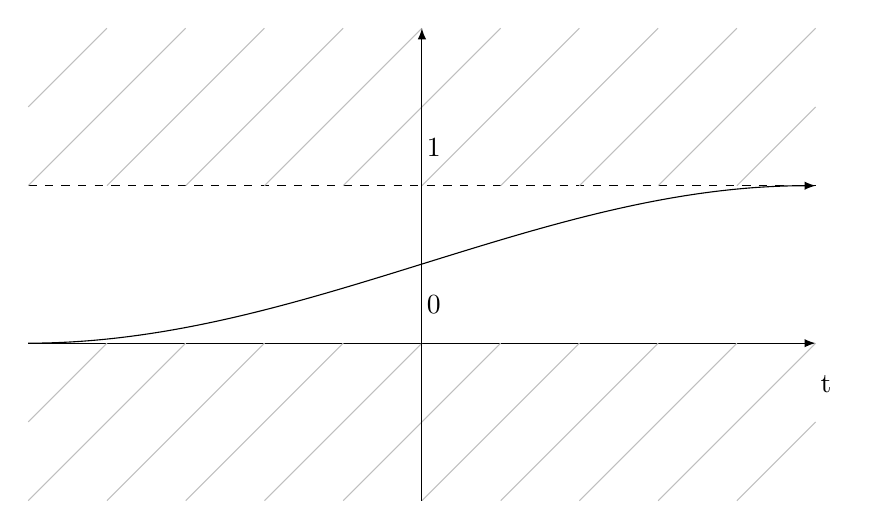
\begin{tikzpicture}
		\draw[draw=black, -latex, thin, solid] (-5.00,0.00) -- (5.00,0.00);
		\node[black, anchor=south west] at (4.94,-0.75) {t};
		\node[black, anchor=south west] at (-0.06,2.25) {1};
		\draw[draw=black, thin, dashed] (-5.00,2.00) -- (5.00,2.00);
		\draw[draw=lightgray, thin, solid] (-5.00,3.00) -- (-4.00,4.00);
		\draw[draw=lightgray, thin, solid] (-5.00,2.00) -- (-3.00,4.00);
		\draw[draw=lightgray, thin, solid] (-4.00,2.00) -- (-2.00,4.00);
		\draw[draw=lightgray, thin, solid] (-3.00,2.00) -- (-1.00,4.00);
		\draw[draw=lightgray, thin, solid] (-2.00,2.00) -- (0.00,4.00);
		\draw[draw=lightgray, thin, solid] (-1.00,2.00) -- (1.00,4.00);
		\draw[draw=lightgray, thin, solid] (0.00,2.00) -- (2.00,4.00);
		\draw[draw=lightgray, thin, solid] (1.00,2.00) -- (3.00,4.00);
		\draw[draw=lightgray, thin, solid] (2.00,2.00) -- (4.00,4.00);
		\draw[draw=lightgray, thin, solid] (3.00,2.00) -- (5.00,4.00);
		\draw[draw=lightgray, thin, solid] (4.00,2.00) -- (5.00,3.00);
		\draw[draw=lightgray, thin, solid] (-5.00,-1.00) -- (-4.00,0.00);
		\draw[draw=lightgray, thin, solid] (-5.00,-2.00) -- (-3.00,0.00);
		\draw[draw=lightgray, thin, solid] (-4.00,-2.00) -- (-2.00,0.00);
		\draw[draw=lightgray, thin, solid] (-3.00,-2.00) -- (-1.00,0.00);
		\draw[draw=lightgray, thin, solid] (-2.00,-2.00) -- (0.00,0.00);
		\draw[draw=lightgray, thin, solid] (-1.00,-2.00) -- (1.00,0.00);
		\draw[draw=lightgray, thin, solid] (0.00,-2.00) -- (2.00,0.00);
		\draw[draw=lightgray, thin, solid] (1.00,-2.00) -- (3.00,0.00);
		\draw[draw=lightgray, thin, solid] (2.00,-2.00) -- (4.00,0.00);
		\draw[draw=lightgray, thin, solid] (3.00,-2.00) -- (5.00,0.00);
		\draw[draw=lightgray, thin, solid] (4.00,-2.00) -- (5.00,-1.00);
		\draw[draw=black, -latex, thin, solid] (0.00,-2.00) -- (0.00,4.00);
		\draw[draw=black, thin, -latex, solid] (-5.00,0.00) .. controls (-1.50, 0.00) and (1.50, 2.00) .. (5.00,2.00);
		\node[black, anchor=south west] at (-0.06,0.25) {0};
	\end{tikzpicture}
\end{center}

\begin{itemize}
	\item $F_X(t)$ è sempre debolmente monotona, ossia $t_1<t_2, F_X(t_1)\leqslant F_X(t_2)$.
	\item Non ci chiederemo la probabilità di valori esatti ma di intervalli. \[P(a<x\leqslant b)=P(x\leqslant b)-P(x\leqslant a)\] Più $b$ è vicino ad'$a$ più la probabilità tende a 0, quindi $P(x=t)=0, \forall t \in \mathbb{R}$.
\end{itemize}

\definizione{Densità di variabile continua}{Sia $F_X(s)$ una funzione e si dice densità di $X$ se $\forall a,b\mid a<b$ si ha \[P(a<x<b)=\int_a^bf_X(s)ds\]}{d:densVarCont}

L'area sotto il grafico tra $a$ e $b$ è la probabilità.

\[\int_a^bf_X(s)ds=F_X(b)-F_X(a)\]

$F$ è primitiva di $f$, quindi $F_X'=f_X$.

\[F_X(t)=\int_{-\infty}^tf_X(s)ds\]

\definizione{Densità continua uniforme}{$X$ si dice uniforme in un intervallo $[a,b]$ se la densità di $X$ è constante in $[a,b]$ e nulla al di fuori di $[a,b]$.

\begin{center}
	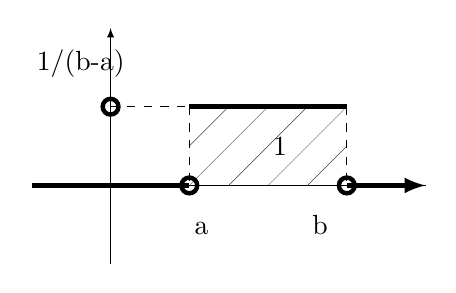
\begin{tikzpicture}
		\draw[draw=black, very thin, solid] (-1.00,0.00) -- (4.00,0.00);
		\draw[draw=black, -latex, very thin, solid] (0.00,-1.00) -- (0.00,2.00);
		\draw[draw=black, ultra thick, solid] (1.00,1.00) -- (3.00,1.00);
		\draw[draw=black, ultra thick, solid] (-1.00,0.00) -- (1.00,0.00);
		\draw[draw=black, -latex, ultra thick, solid] (3.00,0.00) -- (4.00,0.00);
		\node[black, anchor=south west] at (0.94,-0.75) {a};
		\node[black, anchor=south west] at (2.44,-0.75) {b};
		\draw[draw=black, ultra thick, solid] (1.00,0.00) circle (0.1);
		\draw[draw=black, ultra thick, solid] (3.00,0.00) circle (0.1);
		\draw[draw=black, thin, dashed] (1.00,1.00) -- (1.00,0.00);
		\draw[draw=black, thin, dashed] (3.00,1.00) -- (3.00,0.00);
		\draw[draw=black, ultra thin, solid] (1.00,0.00) -- (2.00,1.00);
		\draw[draw=black, ultra thin, solid] (2.00,0.00) -- (3.00,1.00);
		\draw[draw=black, ultra thin, solid] (1.50,0.00) -- (2.50,1.00);
		\draw[draw=black, ultra thin, solid] (1.00,0.50) -- (1.50,1.00);
		\draw[draw=black, ultra thin, solid] (2.50,0.00) -- (3.00,0.50);
		\draw[draw=black, very thin, dashed] (0.00,1.00) -- (1.00,1.00);
		\node[black, anchor=south west] at (-1.06,1.25) {1/(b-a)};
		\draw[draw=black, ultra thick, solid] (0.00,1.00) circle (0.1);
		\node[black, anchor=south west] at (1.94,0.25) {1};
	\end{tikzpicture}
\end{center}}{d:densContUnif}

\osservazione{Siccome $P(-\infty<x<+\infty)=1$ l'area compresa tra il grafico della densità e l'asse orrizontale è sempre 1.}

\osservazione{$X$ è uniforme in $[a,b]$ nel senso che $\forall a_1, b_1, a_2, b_2$ con $b_1-a_1=b_2-a_2=l$. \[P(a_1<x<b_1)=P(a_2<x<b_2)=\frac{l}{b-a}\]}

\mysubsection{Confronto Probabilità discretà e continua}
\begin{align*}
	X&\sim B(3,\frac{1}{2})\\
	d_X(k&)=\begin{cases}
		\frac{1}{8}\ se \ k=0,3\\
		\frac{3}{8}\ se \ k=1,2\\
		0\ altrimenti
	\end{cases}
\end{align*}
\begin{center}
	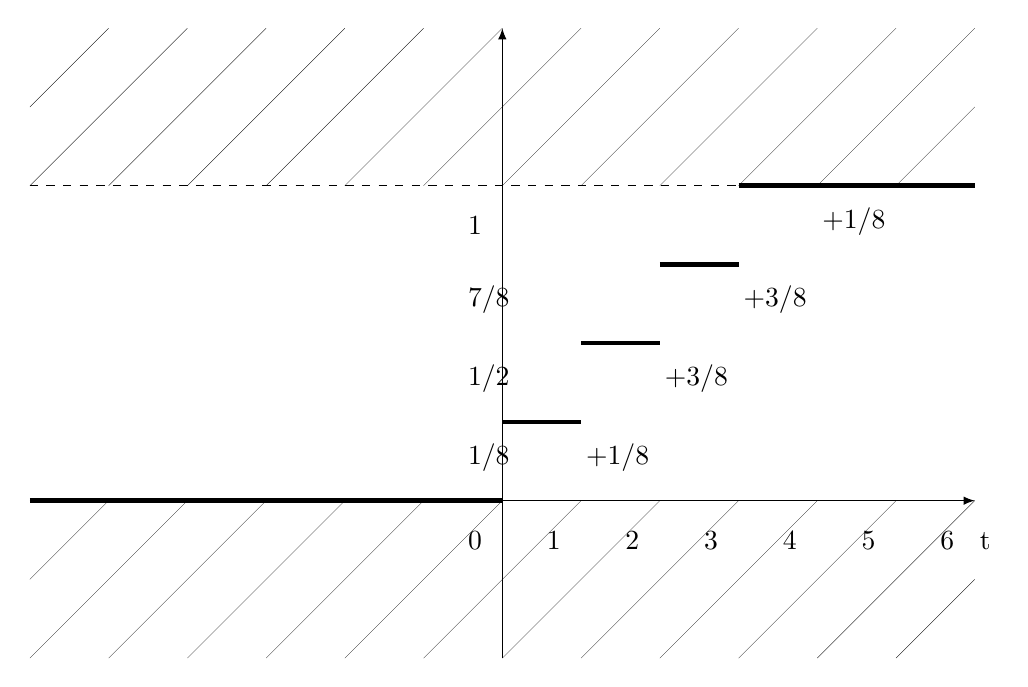
\begin{tikzpicture}
		\draw[draw=black, -latex, thin, solid] (-6.00,0.00) -- (6.00,0.00);
		\node[black, anchor=south west] at (5.94,-0.75) {t};
		\draw[draw=black, -latex, thin, solid] (0.00,-2.00) -- (0.00,6.00);
		\draw[draw=black, thin, dashed] (-6.00,4.00) -- (6.00,4.00);
		\draw[draw=black, ultra thin, solid] (-6.00,5.00) -- (-5.00,6.00);
		\draw[draw=black, ultra thin, solid] (-6.00,4.00) -- (-4.00,6.00);
		\draw[draw=black, ultra thin, solid] (-5.00,4.00) -- (-3.00,6.00);
		\draw[draw=black, ultra thin, solid] (-4.00,4.00) -- (-2.00,6.00);
		\draw[draw=black, ultra thin, solid] (-3.00,4.00) -- (-1.00,6.00);
		\draw[draw=black, ultra thin, solid] (-2.00,4.00) -- (0.00,6.00);
		\draw[draw=black, ultra thin, solid] (-1.00,4.00) -- (1.00,6.00);
		\draw[draw=black, ultra thin, solid] (0.00,4.00) -- (2.00,6.00);
		\draw[draw=black, ultra thin, solid] (1.00,4.00) -- (3.00,6.00);
		\draw[draw=black, ultra thin, solid] (2.00,4.00) -- (4.00,6.00);
		\draw[draw=black, ultra thin, solid] (3.00,4.00) -- (5.00,6.00);
		\draw[draw=black, ultra thin, solid] (4.00,4.00) -- (6.00,6.00);
		\draw[draw=black, ultra thin, solid] (5.00,4.00) -- (6.00,5.00);
		\draw[draw=black, ultra thin, solid] (-6.00,-1.00) -- (-5.00,0.00);
		\draw[draw=black, ultra thin, solid] (-6.00,-2.00) -- (-4.00,0.00);
		\draw[draw=black, ultra thin, solid] (-5.00,-2.00) -- (-3.00,0.00);
		\draw[draw=black, ultra thin, solid] (-4.00,-2.00) -- (-2.00,0.00);
		\draw[draw=black, ultra thin, solid] (-2.00,-2.00) -- (0.00,0.00);
		\draw[draw=black, ultra thin, solid] (-1.00,-2.00) -- (1.00,0.00);
		\draw[draw=black, ultra thin, solid] (0.00,-2.00) -- (2.00,0.00);
		\draw[draw=black, ultra thin, solid] (1.00,-2.00) -- (3.00,0.00);
		\draw[draw=black, ultra thin, solid] (2.00,-2.00) -- (4.00,0.00);
		\draw[draw=black, ultra thin, solid] (3.00,-2.00) -- (5.00,0.00);
		\draw[draw=black, ultra thin, solid] (4.00,-2.00) -- (6.00,0.00);
		\draw[draw=black, ultra thin, solid] (5.00,-2.00) -- (6.00,-1.00);
		\draw[draw=black, ultra thin, solid] (-3.00,-2.00) -- (-1.00,0.00);
		\node[black, anchor=south west] at (-0.56,-0.75) {0};
		\node[black, anchor=south west] at (0.44,-0.75) {1};
		\node[black, anchor=south west] at (1.44,-0.75) {2};
		\node[black, anchor=south west] at (2.44,-0.75) {3};
		\node[black, anchor=south west] at (3.44,-0.75) {4};
		\node[black, anchor=south west] at (4.44,-0.75) {5};
		\node[black, anchor=south west] at (5.44,-0.75) {6};
		\node[black, anchor=south west] at (-0.56,0.25) {1/8};
		\node[black, anchor=south west] at (-0.56,1.25) {1/2};
		\node[black, anchor=south west] at (-0.56,2.25) {7/8};
		\node[black, anchor=south west] at (-0.56,3.25) {1};
		\draw[draw=black, ultra thick, solid] (-6.00,0.00) -- (0.00,0.00);
		\draw[draw=black, ultra thick, solid] (0.00,1.00) -- (1.00,1.00);
		\draw[draw=black, ultra thick, solid] (1.00,2.00) -- (2.00,2.00);
		\draw[draw=black, ultra thick, solid] (2.00,3.00) -- (3.00,3.00);
		\draw[draw=black, ultra thick, solid] (3.00,4.00) -- (6.00,4.00);
		\node[black, anchor=south west] at (0.94,0.25) {+1/8};
		\node[black, anchor=south west] at (1.94,1.25) {+3/8};
		\node[black, anchor=south west] at (2.94,2.25) {+3/8};
		\node[black, anchor=south west] at (3.94,3.25) {+1/8};
	\end{tikzpicture}
\end{center}
\begin{align*}
	P(x\leqslant a)&=\int_{-\infty}^af_X(s)ds=0\\
	P(x\leqslant1)&=1\\
	F_X(t)&=P(X\leqslant t)=\int_a^t\frac{1}{b-a}ds=\frac{t-a}{b-a}
\end{align*}
\begin{center}
		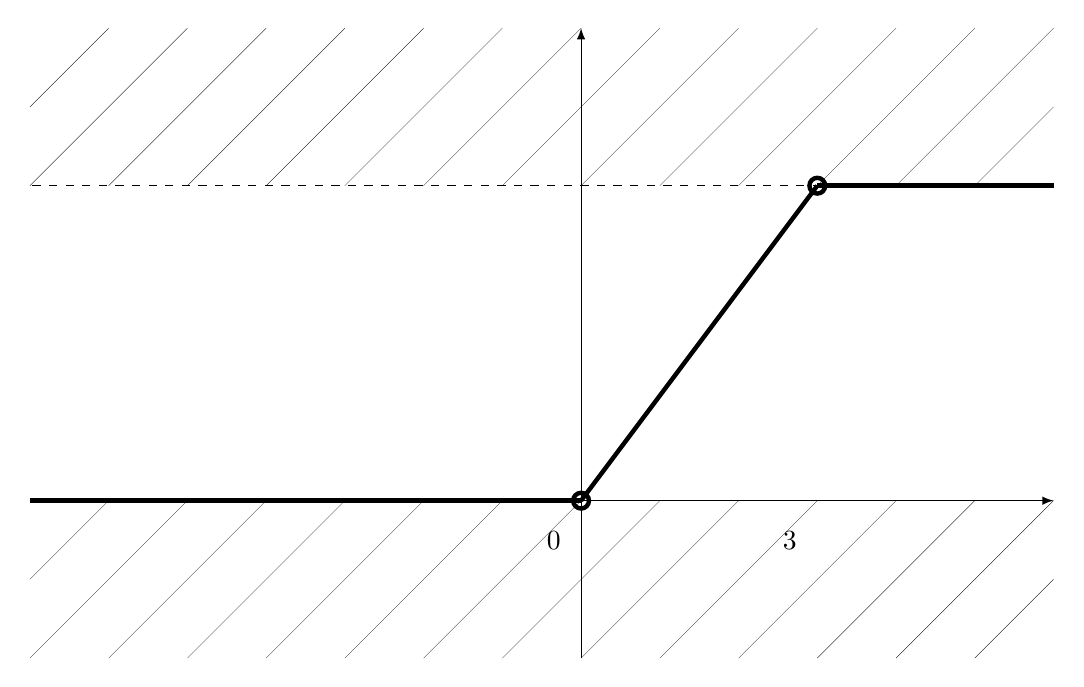
\begin{tikzpicture}
			\draw[draw=black, -latex, thin, solid] (-7.00,0.00) -- (6.00,0.00);
			\draw[draw=black, -latex, thin, solid] (0.00,-2.00) -- (0.00,6.00);
			\draw[draw=black, very thin, dashed] (6.00,4.00) -- (-7.00,4.00);
			\draw[draw=black, ultra thin, solid] (-7.00,5.00) -- (-6.00,6.00);
			\draw[draw=black, ultra thin, solid] (-7.00,4.00) -- (-5.00,6.00);
			\draw[draw=black, ultra thin, solid] (-6.00,4.00) -- (-4.00,6.00);
			\draw[draw=black, ultra thin, solid] (-5.00,4.00) -- (-3.00,6.00);
			\draw[draw=black, ultra thin, solid] (-4.00,4.00) -- (-2.00,6.00);
			\draw[draw=black, ultra thin, solid] (-3.00,4.00) -- (-1.00,6.00);
			\draw[draw=black, ultra thin, solid] (-2.00,4.00) -- (0.00,6.00);
			\draw[draw=black, ultra thin, solid] (-1.00,4.00) -- (1.00,6.00);
			\draw[draw=black, ultra thin, solid] (0.00,4.00) -- (2.00,6.00);
			\draw[draw=black, ultra thin, solid] (1.00,4.00) -- (3.00,6.00);
			\draw[draw=black, ultra thin, solid] (-7.00,-1.00) -- (-6.00,0.00);
			\draw[draw=black, ultra thin, solid] (-7.00,-2.00) -- (-5.00,0.00);
			\draw[draw=black, ultra thin, solid] (-6.00,-2.00) -- (-4.00,0.00);
			\draw[draw=black, ultra thin, solid] (-5.00,-2.00) -- (-3.00,0.00);
			\draw[draw=black, ultra thin, solid] (-4.00,-2.00) -- (-2.00,0.00);
			\draw[draw=black, ultra thin, solid] (-3.00,-2.00) -- (-1.00,0.00);
			\draw[draw=black, ultra thin, solid] (-2.00,-2.00) -- (0.00,0.00);
			\draw[draw=black, ultra thin, solid] (-1.00,-2.00) -- (1.00,0.00);
			\draw[draw=black, ultra thin, solid] (0.00,-2.00) -- (2.00,0.00);
			\draw[draw=black, ultra thin, solid] (1.00,-2.00) -- (3.00,0.00);
			\draw[draw=black, ultra thin, solid] (2.00,4.00) -- (4.00,6.00);
			\draw[draw=black, ultra thin, solid] (3.00,4.00) -- (5.00,6.00);
			\draw[draw=black, ultra thin, solid] (4.00,4.00) -- (6.00,6.00);
			\draw[draw=black, ultra thin, solid] (5.00,4.00) -- (6.00,5.00);
			\draw[draw=black, ultra thin, solid] (2.00,-2.00) -- (4.00,0.00);
			\draw[draw=black, ultra thin, solid] (3.00,-2.00) -- (5.00,0.00);
			\draw[draw=black, ultra thin, solid] (4.00,-2.00) -- (6.00,0.00);
			\draw[draw=black, ultra thin, solid] (5.00,-2.00) -- (6.00,-1.00);
			\draw[draw=black, ultra thick, solid] (0.00,0.00) circle (0.1);
			\draw[draw=black, ultra thick, solid] (3.00,4.00) circle (0.1);
			\draw[draw=black, ultra thick, solid] (0.00,0.00) -- (3.00,4.00);
			\draw[draw=black, ultra thick, solid] (3.00,4.00) -- (6.00,4.00);
			\draw[draw=black, ultra thick, solid] (-7.00,0.00) -- (0.00,0.00);
			\node[black, anchor=south west] at (-0.56,-0.75) {0};
			\node[black, anchor=south west] at (2.44,-0.75) {3};
		\end{tikzpicture}
\end{center}

\definizione{Funzione di ripartizione astratta}{Una funzione $F:\mathbb{R}\to\mathbb{R}$ si dice funzione di ripartizione astratta se:
\begin{enumerate}
	\item $F$ è una funzione continua.
	\item $\lim\limits_{t\to-\infty}F(t)=0, \lim\limits_{t\to+\infty}F(t)=1$.
	\item $F_X$ è debolmente crescente, cioé $\forall t_1<t_2, F(t_1)\leqslant F(t_2)$.
\end{enumerate}}{d:funzRipAstr}

\definizione{Densità continua}{Una funzione $f_X(s)$ si dice densità continua di $X$ se $\forall a,b$ con $a<b$ si ha \[P(a<X<b)=\int_{a}^{b}f_X(s)ds\]}{d:densCont}

\definizione{Densità continua astratta}{Una funzione $f:\mathbb{R}\to\mathbb{R}$ si dice densità continua astratta se:
\begin{enumerate}
	\item $f(s)\geqslant0,\forall s \in \mathbb{R}$.
	\item $\int_{-\infty}^{\infty}f(s)ds=1$.
\end{enumerate}}{d:densContAstr}

\begin{figure}[H]
	\centering
	\includegraphics[width=0.5\textwidth]{img/confronto.png}
	\caption{Descrizione}
\end{figure}

\definizione{Valore atteso di V.A. Contimua}{Il valore atteso di una variabile aletoria continua $X$ è \[E[X]=\int_{-\infty}^{\infty}sf_X(s)ds\]}{d:valAttVaCont}

\osservazione{Il valore atteso di $X\sim U\{[a,b]\}$ è $\frac{a+b}{2}$.}

\proprieta{Valore Atteso V.A. Continua}{
\begin{enumerate}
	\item E' sempre lineare \[E[aX+bY]=aE[X]+bE[y]\]
	\item Siano $X,Y$ indipendenti, allora \[E[XY]=E[X]E[Y]\].
	\item Sia $\Phi:\mathbb{R}\to\mathbb{R}$ una trasformazione allora \[E[\Phi(X)]=\int_{-\infty}^{\infty}\Phi(s)f_X(s)ds\].
\end{enumerate}}{prop:vac}

\definizione{Varianza V.A. Continua}{Sia $X$ una variabile aleatoria continua, allora \[\mathrm{Var}(X)=E[(X-E[X])^2]\] \[\mathrm{Var}(X)=E[X^2]-E[X]^2\]}{def:varVac}

\osservazione{La varianza dipende dall'ampiezza dell'interallo.}

\proprieta{Varianza V.A. Continua}{
\begin{enumerate}
	\item $\mathrm{Var}(aX)=a^2\mathrm{Var}(X)$.
	\item Siano $X,Y$ indipendenti, allora \[\mathrm{Var}(X+Y)=\mathrm{Var}(X)+\mathrm{Var}(Y)\]
\end{enumerate}}{prop:varVac}

\definizione{Variabile esponenziale}{Sia $a>0$, allora $X\sim Exp(a)$ si definisce \[f(s)=\begin{cases}
		0 \ se \ s<0\\
		ae^{-as} \ se \ s>0
\end{cases}\]
$f(s)$ è una densità continua astratta.}{d:varEsp}

\[f(s)\geqslant0,\forall s\]
\begin{center}
	\begin{tikzpicture}
		\draw[draw=black, -latex, thin, solid] (-5.00,0.00) -- (5.00,0.00);
		\draw[draw=black, -latex, thin, solid] (0.00,-1.00) -- (0.00,4.00);
		\draw[draw=magenta, thin, solid] (0.00,3.00) .. controls (0.50, 0.50) and (0.50, 0.50) .. (5.00,0.00);
		\node[black, anchor=south west] at (-0.56,-0.75) {0};
		\node[black, anchor=south west] at (-0.56,2.25) {a};
		\node[black, anchor=south west] at (4.44,-0.75) {t};
		\draw[draw=black, thin, solid] (0.00,0.00) circle (0.1);
		\draw[draw=black, thin, solid] (0.00,3.00) circle (0.1);
		\draw[draw=magenta, thin, solid] (-5.00,0.00) -- (0.00,0.00);
	\end{tikzpicture}
\end{center}

La funzione di ripartizione è \[F_X(t)=\int_{-\infty}^{t}f(s)ds=\begin{cases}
	0 \ se \ t\leqslant0\\
	1-e^{-at} \ se \ t>0
\end{cases}\]

\begin{center}
	\begin{tikzpicture}
		\draw[draw=black, -latex, thin, solid] (-5.00,0.00) -- (5.00,0.00);
		\draw[draw=black, -latex, thin, solid] (0.00,-1.00) -- (0.00,4.00);
		\draw[draw=black, thin, dashed] (-5.00,3.00) -- (5.00,3.00);
		\node[black, anchor=south west] at (-0.56,-0.75) {0};
		\node[black, anchor=south west] at (-0.56,2.25) {1};
		\draw[draw=black, thin, dashed] (0.00,0.00) circle (0.1);
		\draw[draw=red, thin, solid] (0.00,0.00) .. controls (0.50, 2.50) and (0.50, 2.50) .. (5.00,3.00);
		\draw[draw=red, thin, solid] (-5.00,0.00) -- (0.00,0.00);
		\node[red, anchor=south west] at (4.44,-0.75) {t};
	\end{tikzpicture}
\end{center}

Le variabili esponenziali hanno \textbf{mancanza di memoria} \[P(X\geqslant t+s\mid X\geqslant t)=P(X\geqslant s)\]

Sapendo che $P(X\geqslant t)=1-P(X\leqslant t)=1-(1-e^{-at})=e^{-at}$ per $(t>0)$.

Dimostrazione:
\begin{align*}
	P(X\geqslant t+s\mid X \geqslant t)&=\frac{P(X\geqslant t+s, X\geqslant t)}{P(X\geqslant t)}\\
	&= \frac{e^{-a(t+s)}}{e^{-at}}=e^{-as}=P(X\geqslant s)
\end{align*}

Questa proprietà comporta che le variabili esponenziali modellizzano il tempo d'attesa di un fenomeno naturale.

Il valore atteso è $E[X]=\frac{1}{a}$. La varianza è $\mathrm{Var}(X)=\frac{1}{a^2}$.

\definizione{Trasformazioni di Variabili Aleatorie Continue}{Sia $\Phi:\mathbb{R}\to\mathbb{R}$ una trasformazione e $X$ una variabile aleatoria continua, allora $\Phi(X)$ è la trasformazione della variabile aleatoria continua $X$.

La funzione di ripartizione sarà \[F_{\Phi(X)}(t)=P(\Phi(X)\leqslant t)\]}{d:trasVAC}

Negli esercizi si risolve la diseguaglianza e si esprime la $F_{\Phi(X)}$ in $F_X$.

\definizione{Variabili normali (Gaussiane)}{Siano l'integrale di Gauss e la rispettiva densità astratta.
Non esiste una formula per $F(s)$ (funzione di ripartizione), quindi per $0<t<4$ si usano valori noti detti $\phi(t)$.
\[\int_{-\infty}^{\infty}e^{\frac{-s^2}{2}}ds=\sqrt{2\pi}\]
\[f(s)=\frac{1}{\sqrt{2\pi}}e^{\frac{-s^2}{2}}\]
Una variabile con questa densità la chiamiamo normale standard e la indichiamo $ \zeta_0$. Scriviamo $\zeta_0\sim N(0,1)$.}{def:varGaussiane}

Densità di $\zeta_0$:
\begin{figure}[H]
	\centering
	\includegraphics[width=0.5\textwidth]{img/gauss.png}
	\caption{Descrizione}
\end{figure}

\mysubsection{Somma opposti}
Chiamiamo $\Phi(t)=F_{\zeta_o}(t)$. Siano $\Phi(t)\cong1$ se $t>4$ e $\Phi(t)\cong0$ se $t<-4$, allora \[\Phi(t)+\Phi(-t)=1\]

\begin{figure}[H]
	\centering
	\includegraphics[width=0.5\textwidth]{img/sommaOpposti.png}
	\caption{Descrizione}
\end{figure}

\mysubsection{Valore atteso e Varianza Variabile Normale}
Per simmetria della densità si ha valore atteso 0. \[E[\zeta_0]=0\]

La varianza vale 1 dato che il valore atteso del quadrato vale 1. \[\mathrm{Var}(\zeta_0)=1\]

\definizione{Variabili Normali non Standard}{Dati $\mu$ e $\delta>0$ la variabile $\zeta\sim N(\mu,\delta^2)$ è data da \[\zeta=\mu+\delta\zeta_0\]

$E[\zeta]=\mu$, $\mathrm{Var}(\zeta)=\delta^2$.}{d:varNormNonStand}

In pratica $\mu>0$ slide a destra, $\mu<0$ slide a sinistra, $\sigma>1$ funzione "spanciata", $\delta<0$ funzione "compatta".

\textbf{Standardizzazione}: Dato $\zeta\sim N(a,b)$ si ottiene $\zeta=a+\sqrt{b}\zeta_0$ di cui si calcola la probabilità $P(\zeta\gtrless c)=P(\zeta_0>\frac{c-a}{b})=1+\Phi(\frac{c-a}{b})$.

\bigskip

\textbf{Scopo?} Le variabili normali sono quelle che si presentano solitamente quando abbiamo a che fare con misurazioni.

\teorema{Teorema Centrale del limite}{Siano $X_1,\dots,X_n$ variabili aleatorie (discrete o continue) aventi la stessa funzione di ripartizione di valore atteso $\mu$ e varianza $\delta^2$ e indipendenti. Allora $X_1+\dots+X_n$ è approssimativamente una variabile normale $N(n\mu,n\delta^2)$. Se $n$ è abbastanza grande.

In generale considerando $\overline{X_n}=\frac{X_1+\dots+X_n}{n}$ si ha $E[\overline{X_n}]=\mu$ e $\mathrm{Var}(\overline{X_n})=\frac{\delta^2}{n}$. Ottenendo cosi $X_n\sim N(\mu, \frac{\delta^2}{n})$.
}{teo:centLim}

\dimostrazione{teo:centLim}{Consideriamo $X\sim U([-1,1])$ di densità:
\begin{figure}[H]
	\centering
	\includegraphics[width=0.5\textwidth]{img/teoCentLim1.png}
	\caption{Descrizione}
\end{figure}
Siano ora $X_1,X_2\sim U([-1,1])$ indipendenti, allora $X_1+X-2$ assume valori tra $[-2,2]$:
\begin{figure}[H]
	\centering
	\includegraphics[width=0.5\textwidth]{img/teoCentLim2.png}
	\caption{Descrizione}
\end{figure}
Analogamente con $X_1,X_2,X_3\sim U([-1,1])$ indipendneti, allora $X_1+X_2+X_3$ assume valori tra $[-3,3]$. (3 rami di parabola).
\begin{figure}[H]
	\centering
	\includegraphics[width=0.5\textwidth]{img/teoCentLim3.png}
	\caption{Descrizione}
\end{figure}
E cosi facendo...}

\bigskip

Dato $c$ con $0<c<1$. La denstià normale standard è data da $P(-Z_c<\zeta_0<Z_c)=\Phi(Z_c)-\Phi(-Z_c)=\Phi(Z_c)-(1-\Phi(Z_c))=2\Phi(Z_c)-1-c=\Phi(Z_c)=\frac{c+1}{2}$.

Sostituendo $\zeta_0$ con $\frac{\overline{X_n}-\mu}{\delta/\sqrt{n}}$ abbiamo $P(-Z_c<\frac{\overline{X_n}-\mu}{\delta/\sqrt{n}}<Z_c)=c$.

\definizione{Correzione di Continuità}{Se le variabili $X_1,\dots,X_n$ assumono valori interi, anche la loro somma darà un valore intero. In questo caso si usa la correzione di continuità in cui un numero intero $n$ viene pensato come l'intervallo \[\left[n-\frac{1}{2}, n+\frac{1}{2}\right]\]}{def:correzioneContinuita}